\chapter{Marco teórico}

\section{Estructura estelar newtoniana}
Se presentarán las ecuaciones de estructura estelar newtonianas para facilitar la interpretación de las ecuaciones de estructura que se obtendrán en Relatividad General.

Considerando una distribución de materia con simetría esférica, si $r$ denota la distancia desde el centro de la configuración, la masa encerrada en una superficie esférica de radio $r$ será:  
\begin{equation}
    m ( r ) = \int _ { 0 } ^ { r } 4 \pi r ^ { 2 } \rho \dd{r} = \int_{0}^{r} \dd{m(r)} \quad\text{con}\quad \dd{m(r)}=4\pi r^2\rho \dd{r},
    \label{mN}
\end{equation}

\begin{equation}
    \Longrightarrow\dv{m(r)}{r} =4\pi r^2 \rho.
    \label{dmnewton}
\end{equation}
Ahora, se considera un cilindro infinitesimal a una distancia $r$ del centro, de altura $\dd{r}$ y sección transversal unitaria, normal al vector posición $\vec{r}$ (ver Figura \ref{stellnew}).  

\begin{figure}[H]
    \centering
    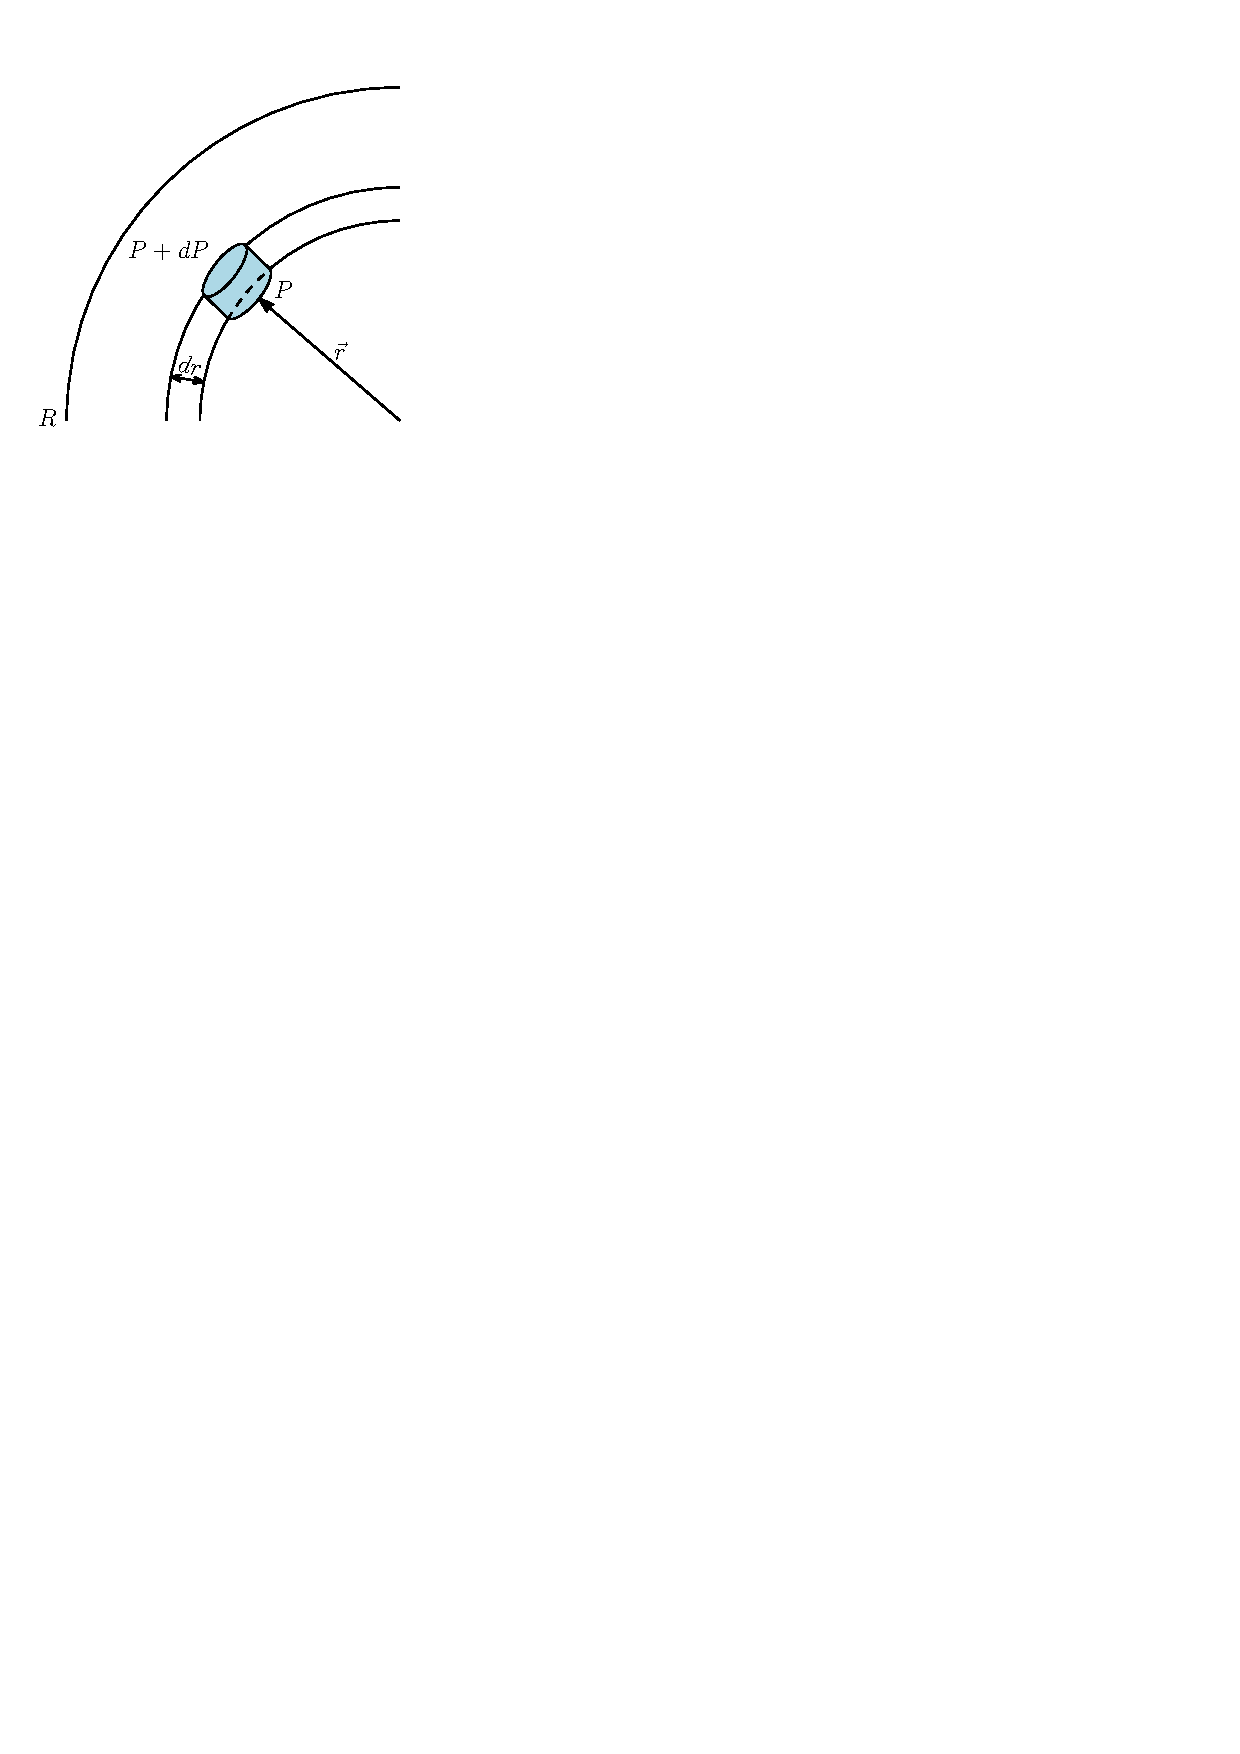
\includegraphics[width=150pt]{figures/stellarnewton.pdf}
    \caption{Presión sobre un elemento de masa cilíndrico.}
    \label{stellnew}
\end{figure}
Si la presión en $\vec{r}$ es $P$ y su cambio al ir de $\vec{r}$ a $\vec{r}+\dd{\vec{r}}$ es $\dd{P}$. Suponiendo que el elemento de área es $dA$ la diferencia de presión representa una fuerza 
\begin{equation*}
    F_{Pelem}=-\dd{P}\dd{A},
\end{equation*}
actuando sobre el elemento de masa. Esta fuerza debe contrarrestar la atracción gravitacional sobre el elemento de masa debido a $m(r)$
\begin{equation*}
    F_{atracc}=\frac{G m(r)\rho \dd{A} \dd{r}}{r^2}.
\end{equation*}
Para que el elemento de masa se encuentre en equilibrio se requiere entonces:

\begin{equation}
    -\dd{P}\dd{A} =\frac{G m(r)\rho \dd{A} \dd{r}}{r^2},
\end{equation}
o
\begin{equation}
    \dv{P}{r} = - \frac { G m ( r ) } { r ^ { 2 } } \rho.
    \label{dpnewton}
\end{equation}
que es la conocida ecuación de equilibrio hidrostático. 

Las ecuaciones \eqref{dmnewton} y \eqref{dpnewton} son las ecuaciones de estructura estelar newtonianas \cite{Chandrasekhar1958}. Si una relación entre la presión y la densidad $P(\rho)$ es dada, es decir, una ecuación de estado, el sistema puede resolverse dado un par condiciones iniciales $m(r=0)$ y $P(r=0)$. La primera de estas condiciones es evidente puesto que no hay masa encerrada en un cascarón esférico de radio nulo, $m(r=0)=0$. La segunda estará definida por el valor de $\rho(r=0)\equiv\rho_c$ escogido, mediante la ecuación de estado, $P(r=0)=P(\rho_c)$.

El radio de la estrella $R$ se define como el valor de $r$ en el que la presión se anula, esto es, $P(R)=0$ y de manera similar la masa de la estrella $M$ se define como el valor de la masa encerrada en $r=R$, esto es, $m(R)=M$.

Aunque no se van a tratar en el trabajo de grado, cabe resaltar que las enanas blancas son bien descritas por las ecuaciones de estructura newtonianas. Una manera, aunque no la única, de conocer la importancia de las correcciones relativistas es comparando el valor de $\frac{2GM}{c^2R}$ con la unidad (la razón será evidente en el resultado relativista) \cite{Weinberg1972}. Las enanas blancas tienen masas en un rango de $0.33\,M_{\odot}$ $1.52\,M_{\odot}$ y radios típicos de unos cuantos miles de kilómetros \cite{Glendenning2000}. Para una enana blanca promedio, con masa $M=0.6\,M_{\odot}$ y radio $r=3000 \,\rm{km}$ se tiene
\begin{equation}
    \frac{2GM}{c^2R}\simeq 6\times 10^{-4}\ll 1,
\end{equation}
por lo cual se espera que el tratamiento newtoniano sea suficiente. 

\section{Estructura estelar relativista}

Si bien en la teoría newtoniana podrían existir objetos tan compactos como las estrellas de neutrones, algunas de las predicciones presentan inconsistencias con lo predicho por la teoría de la Relatividad General. Por ejemplo, Chandrasekhar encontró (usando gravedad newtoniana) que las estrellas soportadas por presión de degeneración tienen una masa máxima, obtenida asintóticamente cuando los fermiones son altamente relativistas. Esto es, cuando tienen velocidades comparables con la velocidad de la luz. Bajo tales condiciones la teoría newtoniana permitiría la existencia de estrellas compuestas por los quarks más pesados (charm, bottom y top). En Relatividad General se predice también la existencia de una masa máxima, pero ésta no es de naturaleza asintótica sino que está inmersa en la forma de las ecuaciones de estructura estelar. Las estrellas con la mayor masa posible en Relatividad General, en contraste a lo predicho por la teoría newtoniana, no son lo suficientemente densas para permitir la presencia de los quarks más pesados \cite{Glendenning2000}.

Predicciones contradictorias como la anterior favorecen a la Relatividad General en el estudio de objetos compactos, pues ésta ha explicado fenómenos como la precesión de mercurio, que no pueden ser explicados en gravedad newtoniana (ver  \cite{Turyshev2008ExperimentalRelativity} para una revisión de tests experimentales de la Relatividad General).

Para describir la estructura de una estrella estática en Relatividad General se supone un espacio-tiempo estático e isótropo, descrito de manera general por la métrica:

\begin{equation}
\dd{s}^ { 2 } = e ^ { 2 \nu ( r ) } \dd{ t} ^ { 2 } - e ^ { 2 \lambda ( r ) } \dd{ r} ^ { 2 } - r ^ { 2 } \left( \dd{ \theta} ^ { 2 } + \sin ^ { 2 }  \theta  \dd{ \phi} ^ { 2 } \right) .   
\end{equation}

Además el espacio-tiempo se dividirá en dos: una región exterior a la estrella y una interior. 
La \textit{región exterior} es libre de fuentes ($T _ { \mu } ^ { \nu }=0$) y las ecuaciones de Einstein para ésta, en unidades gravitacionales ($G=c=1$), son 

\begin{equation}
    G _ { \mu } ^ { \nu } = R _ { \mu } ^ { \nu } - \frac { 1 } { 2 } g _ { \mu } ^ { \nu } R = 8 \pi T _ { \mu } ^ { \nu }=0,
\end{equation}
de donde se obtiene
\begin{equation}
    e ^ { 2 \nu } = 1 - \frac { 2 M } { r }\quad \text{y}\quad - e ^ { 2 \lambda } = - e ^ { - 2 \nu } = - \left( 1 - \frac { 2 M } { r } \right) ^ { - 1 },
\end{equation}
donde $M$ es una constante de integración interpretada como la masa de la estrella. Esta es la conocida solución exterior de Schwarzschild
\begin{equation}
    \dd{s} ^ { 2 } =  \left( 1 - \frac { 2 M } { r } \right) \dd{t} ^ { 2 } - \left( 1 - \frac { 2 M } { r } \right) ^ { - 1 } \dd{r} ^ { 2 }  - r ^ { 2 } \dd{\theta} ^ { 2 } - r ^ { 2 } \sin ^ { 2 } \theta \dd{\phi} ^ { 2 }, \label{schwarzs}
\end{equation}
valida para $r>R$, donde $R$ es el radio de la estrella, que describe la geometría del espacio-tiempo por fuera de una estrella estática.

Para la \textit{región interior} el contenido material debe ser especificado para resolver las ecuaciones de Einstein. Si la materia se modela como un fluido perfecto, el tensor de energía-momento viene dado por

\begin{equation}
    \begin{array} { c } { T ^ { \mu \nu } = - P g ^ { \mu \nu } + ( P + \rho ) u ^ { \mu } u ^ { \nu } }, \\ \text{con} \quad { g _ { \mu \nu } u ^ { \mu } u ^ { \nu } = 1 }, \end{array}
\end{equation}
donde $u^{\mu}=\dv{x^{\mu}}{\tau}$ es la cuadri-velocidad de un elemento del fluido. Este tensor puede ser escrito en términos de los valores Minkowskianos de presión $P$ y densidad de energía $\rho$ gracias al Principio de Covariancia (consecuencia del Principio de Equivalencia \cite{Weinberg1972}), que permite escribir el tensor energía-momento en presencia de campos gravitacionales de una manera análoga a como se escribe en relatividad especial en ausencia de gravedad.

Como se considera una estrella estática, la velocidad espacial de todos los elementos del fluido son cero:
\begin{equation}
    u^{i}=0 \quad (i=1,2,3)\qc u ^ { 0 } = 1 / \sqrt { g _ { 00 } }
\end{equation}
con lo que las únicas componentes no nulas del tensor energía-momento, en componentes mixtas, serán

\begin{equation}
T _ { 0 } ^ { 0 } = \rho(r) , \quad T _ { i } ^ { i } = - P(r) \quad ( i=1,2,3 ).  
\end{equation}

Teniendo en cuenta la forma del tensor energía-momento, las ecuaciones de Einstein,

\begin{equation}
    G _ { \mu } ^ { \nu } = R _ { \mu } ^ { \nu } - \frac { 1 } { 2 } g _ { \mu } ^ { \nu } R = 8 \pi T _ { \mu } ^ { \nu },
\end{equation}
serán

\begin{equation}
    \begin{array} { l } { G _ { 0 } ^ { 0 } = e ^ { - 2 \lambda } \left( \frac { 1 } { r ^ { 2 } } - \frac { 2 \lambda ^ { \prime } } { r } \right) - \frac { 1 } { r ^ { 2 } } = - 8 \pi  \rho ( r ) }, \\ { G _ { 1 } ^ { 1 } = e ^ { - 2 \lambda } \left( \frac { 1 } { r ^ { 2 } } + \frac { 2 \nu ^ { \prime } } { r } \right) - \frac { 1 } { r ^ { 2 } } = 8 \pi  P ( r ) }, \\ { G _ { 2 } ^ { 2 } = e ^ { - 2 \lambda } \left( \nu ^ { \prime \prime } + \nu ^ { \prime 2 } - \lambda ^ { \prime } \nu ^ { \prime } + \frac { \nu ^ { \prime } - \lambda ^ { \prime } } { r } \right) = 8 \pi  P ( r ) }, \\ { G _ { 3 } ^ { 3 } = G _ { 2 } ^ { 2 } = 8 \pi  P ( r ) }. \end{array}
    \label{eee}
\end{equation}
Definiendo la masa de Misner como
\begin{equation}
    m ( r ) \equiv 4 \pi \int _ { 0 } ^ { r } \rho ( r ) r ^ { 2 } \dd{r},
    \label{me}
\end{equation}
se puede eliminar las funciones métricas de \eqref{eee}, expresándolas en términos de $P$, $\rho$ y $m$ para obtener 

\begin{equation}
    \dv{P}{r} = - \frac { [ P ( r ) + \rho ( r ) ] \left[ m ( r ) + 4 \pi r ^ { 3 } P ( r ) \right] } { r [ r - 2 m ( r ) ] },
    \label{dptov}
\end{equation}
que junto a \eqref{me}, escrita como

\begin{equation}
    \dv{m}{r} = 4 \pi r ^ { 2 } \rho(r),
    \label{dmtov}
\end{equation}
son las ecuaciones de estructura estelar relativista y son la reducción de las ecuaciones de Einstein para el interior de una estrella esférica y estática. Este sistema es conocido como las ecuaciones de Tolman-Oppenheimer-Volkoff (TOV).

A pesar de que la masa de Misner \eqref{me} tiene la misma forma que la masa newtoniana \eqref{mN}, \eqref{me} incluye la energía total (masa bariónica y energía gravitacional) encerrada dentro de la coordenada $r$. Por esta razón se refiere a $M=m(R)$ como la \emph{masa gravitacional} de la estrella ya que no existe una forma unívoca de calcular la masa dada una distribución de energía arbitraria. 

Re-escribiendo \eqref{dptov} como
\begin{equation}
    \dv{P}{r} =  - \frac { G  m ( r ) } { r ^ { 2 } } \rho ( r ) \left[ 1 + \frac { P ( r ) } {c ^ { 2 } \rho ( r ) } \right] \left[ 1 + \frac { 4 \pi r ^ { 3 } P ( r ) } { m ( r ) c ^ { 2 } } \right]  \left[ 1 - \frac { 2 G m ( r ) } { c ^ { 2 } r } \right] ^ { - 1 }, 
    \label{dprelat}
\end{equation}
donde se revirtió el cambio de unidades, se puede reconocer como una versión relativista de la ecuación de equilibrio hidrostático newtoniana \eqref{dpnewton}. Las cuales coinciden en el límite cuando 
\begin{equation}
    c^2\rho \gg P \qc mc^2 \gg 4\pi r^3P \quad \text{y} \quad  \frac{2Gm}{c^2r}\ll 1.
\end{equation}
Así pues,  \eqref{dprelat} expresa el \textit{balance} entre la fuerza neta sobre un elemento de masa debido a la presión de la materia que la rodea y la atracción gravitacional de la materia interior a este. El hecho de que, además de la densidad de energía, la presión actúe como una fuente de atracción gravitacional es la razón por la cual el colapso gravitacional es intrínseco a la estructura de la Relatividad General pues mientras en las estrellas newtonianas la presión actuaba para sostener a la estrella, si la estrella es lo suficiente masiva (presiones lo suficientemente grandes) el colapso es inevitable.

Las ecuaciones de TOV \eqref{dptov} y \eqref{dmtov}, pueden ser resueltas de manera análoga a las ecuaciones de estructura newtonianas. Dada una ecuación de estado $P(\rho)$ y partiendo de las condiciones iniciales $m(r=0)=0$ y $P(r=0)=P(\rho_c)$, el sistema se puede integrar hasta que la presión se anule, lo que indica el borde de la estrella y define el radio $R$ y la masa gravitacional $m(R)=M$ de la estrella. Los modelos de objetos compactos obtenidos dada cierta ecuación de estado forman una familia parametrizada por la densidad central $\rho_c$. Algunas características generales de la ecuación de estado serán descritas en la siguiente sección.

La función métrica $\nu$ puede ser hallada añadiendo al sistema la ecuación diferencial

\begin{equation}
    \dv{\nu}{r} = \frac { m ( r ) + 4 \pi r ^ { 3 } P ( r ) } { r [ r - 2 m ( r ) ] },
\end{equation}
cuya solución debe coincidir con la solución externa en $R$, por lo que se usa la libertad de sumar una constante para realizar el siguiente cambio
\begin{equation}
    \nu ( r ) \longrightarrow \nu ( r ) - \nu ( R ) + \frac { 1 } { 2 } \ln \left( 1 - \frac { 2 M } { R } \right) , \quad r \leq R.
\end{equation}
Sujeta a una condición inicial, generalmente $\nu(r=0)=0$.

Además, a partir de $\nu$ se puede determinar el corrimiento al rojo gravitacional de señales periódicas \cite{Haensel2007NeutronStructure} como:
\begin{equation}
    z(r)\equiv e^{-\nu(r)}-1.
    \label{redshift}
\end{equation}



\section{Estructura interna y composición de estrellas de neutrones}

La composición de las estrellas de neutrones, contrario a lo que el nombre sugiere, se presume es muy rica y varía a lo largo de su extensión radial, esta variada composición y las distintas fases que exhiben, están distribuidas en una estructura de cascarones, denominada generalmente una red cristalina de Coulomb (ver Figura \ref{NSC}).
La superficie de la estrella está rodeada por una \emph{atmósfera} compuesta principalmente de hidrógeno, helio y hierro (aunque se ha encontrado carbono en una \cite{Ho2009ARemnant}) en estado gaseoso o condensado dependiendo de su temperatura superficial y campo magnético \cite{Zavlin2002ModelingAtmospheres}. La atmósfera es importante porque es donde se forma el espectro de radiación electromagnética y éste aporta información acerca de su composición, temperatura y campo magnético.
Debajo de la atmósfera se encuentra una \emph{envoltura} (de aproximadamente 100 \si{\metre}), a veces llamado océano. Compuesta presuntamente de núcleos alrededor del pico del hierro en un estado condensado, la envoltura influencia el transporte y emisión de energía térmica desde la superficie \cite{Piekarewicz2013,Potekhin,Lattimer2004}.




La envoltura encierra a cuatro regiones internas: la corteza exterior e interior y el núcleo exterior e interior. La \emph{corteza} es una capa en la que se encuentra materia con densidades sub-nucleares ($\rho < \rho_0$). En la \emph{corteza exterior} los electrones presentes, requeridos para la neutralidad de carga de la estrella, forman un gas de Fermi y ocurre un proceso de neutronización donde los electrones son capturados por protones para crear neutrones. La división con la \emph{corteza interior} se presenta debido a que a una densidad $\rho_{ND}\simeq 10^{14}\, \si{\gram\per\centi\metre^2}$ (neutron drip density), los neutrones comienzan a \com{gotear} del núcleo, por lo que hay presencia de neutrones libres, que pueden llegar a condensarse en un superfluido \cite{Baldo2005SuperfluidityMatter}. En el fondo de la corteza, cuando la densidad se acerca a $\rho_0$, se ha predicho la presencia de fases conocidas como \com{pasta} nuclear, en las que, debido a la compresión, los núcleos se deforman y dejan de ser esféricos (para una revisión de la corteza de las estrellas de neutrones consultar \cite{Chamel2008} y referencias allí citadas). 

\begin{figure}[H]
    \centering
    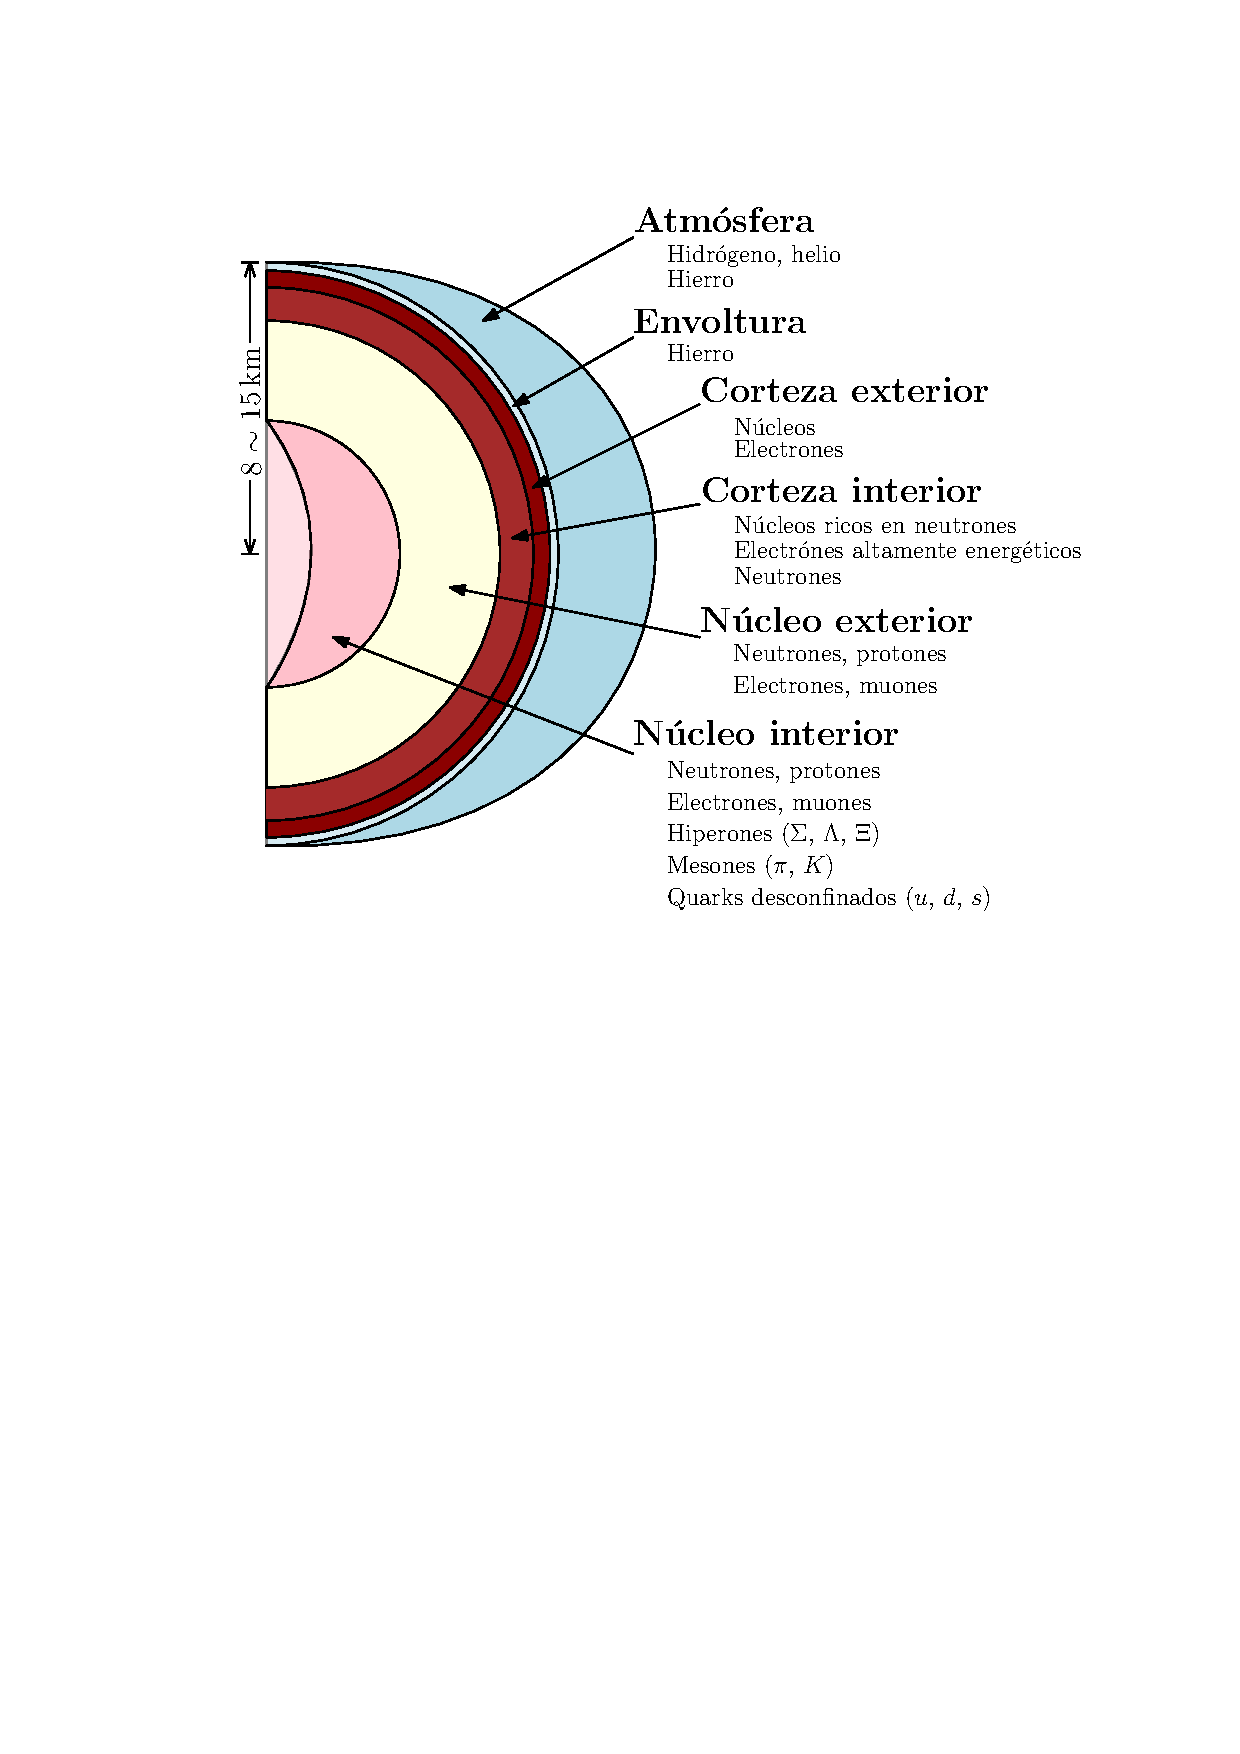
\includegraphics[width=300pt]{figures/neutronstar.pdf}
    \caption{Composición de una estrella de neutrones.\protect\footnotemark}
    \label{NSC}
\end{figure}
\footnotetext{Original: Figura 1 de \cite{Weber2012}}


El \emph{núcleo} comprende regiones en las que la densidad alcanza $\rho_0$ y contiene la mayor fracción de la masa estelar. Está subdividido un dos: el \emph{núcleo exterior}, con densidad $\num{0.5}\rho_0\lesssim\rho\lesssim 2\rho_0$  cuya composición se conoce bien cualitativamente \cite{Haensel2007NeutronStructure}: es un superfluido de neutrones y protones, con presencia de electrones y muones altamente degenerados. Del \emph{núcleo interior}, por el contrario, no se conoce su composición. Se ha sugerido la presencia de hiperones, piones, kaones e incluso quarks desconfinados (consultar las revisiones \cite{Lattimer2004,Potekhin} y referencias allí citadas).



La gran variedad de fases que se encuentran a medida de que la densidad aumenta en el interior de las estrellas de neutrones están ilustradas en la Figura \ref{NSS}. 

   



\subsection{Ecuación de estado}

La composición de la estrella de neutrones entra en el cálculo de la estructura estelar mediante la ecuación de estado $P(\rho)$. Ésta es determinada predominantemente por la interacción nuclear fuerte entre los constituyentes de la materia ultradensa. Las interacciones nucleares son responsables de las características de la ecuación de estado, incluso a densidades menores que $\rho_0$. 

\begin{figure}[H]
    \centering
    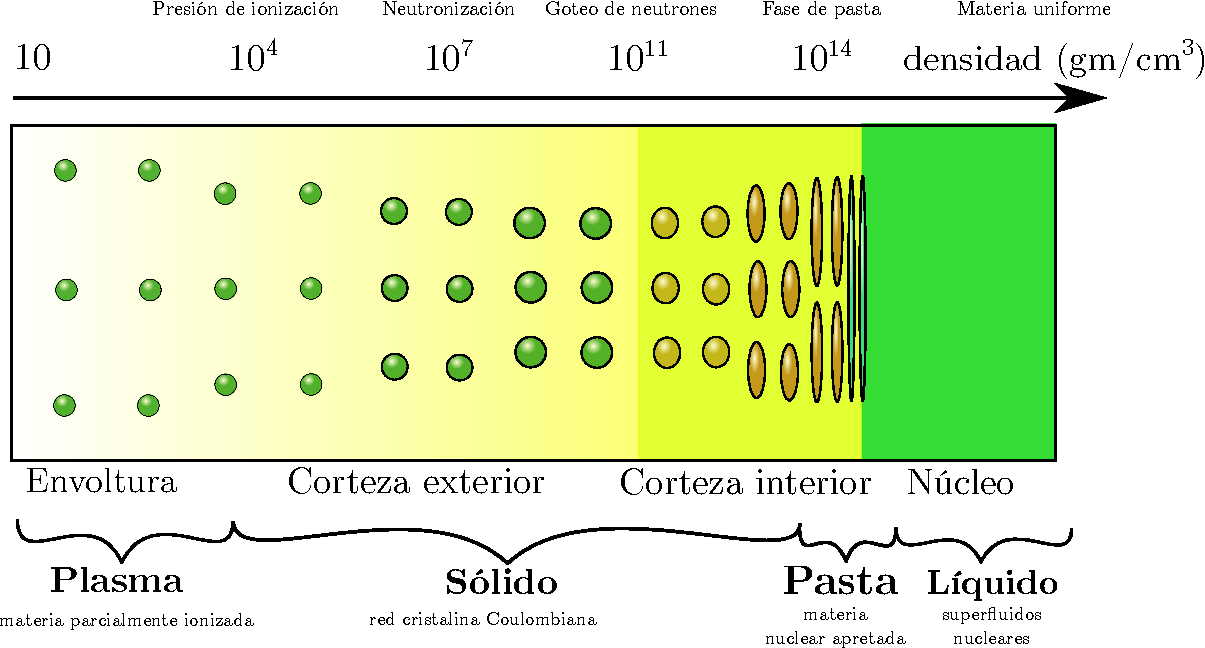
\includegraphics[width=420pt]{figures/Density.pdf}
    \caption[Estructura interna de una estrella de neutrones]{Estructura interna de una estrella de neutrones.\protect\footnotemark}
    \label{NSS}
\end{figure}
\footnotetext{Original: Figura 4 de \cite{Chamel2008}}

Desafortunadamente, aún en regiones con densidades subnucleares, el cálculo de la ecuación de estado comenzando con una interacción nucleón-nucleón (NN) determinada experimentalmente en el vacío, suplementada por una fuerza de tres nucleones (NNN), no es práctica. Esto debido a que el problema de muchos cuerpos es muy complejo en el caso de núcleos pesados. Para que sea posible hacer cálculos, se usa una aproximación de campo medio (mean field approximation) con una interacción NN efectiva \cite{Douchin2001AStructure}. En este esquema, la composición del núcleo estará determinada por la forma precisa de la interacción efectiva NN.
Además, la aproximación de campo medio permite describir de manera consistente la transición entre la corteza interior y el núcleo, usando el mismo modelo de muchos cuerpos y la misma interacción efectiva a ambos lados de la interfaz. Cuando no se hace de esta manera, es necesario realizar un procedimiento de acoplamiento entre las ecuaciones de estado de la corteza y el núcleo, en el que es posible introducir inconsistencias termodinámicas \cite{Fortin2016NeutronState}. 

Si bien la ecuación de estado de la materia ultradensa está sujeta a algunas restricciones de experimentos de baja energía y mediciones de radios y masas de estrellas de neutrones (ver \cite{Ozel2016} para una revisión reciente), no hay acceso a datos experimentales en ese régimen y los candidatos son numerosos. Por esto, la ecuación de estado de la materia ultradensa es uno de los grandes misterios de las estrellas de neutrones. 

Dependiendo de la ecuación de estado escogida, las ecuaciones de TOV \eqref{dmtov} y \eqref{dptov} darán diferentes valores de la masa máxima $M_{max}$ de las estrellas neutrones, cuyo interés astrofísico reside en que traza la línea divisoria entre las estrellas de neutrones y los agujeros negros. El valor preciso de $M_{max}$ influye en la caracterización de remanentes de supernova y el estimado del número estrellas de neutrones y agujeros negros en la galaxia. 

\section{Condiciones de aceptabilidad física}
Para que los modelos de objetos compactos obtenidos sean de interés astrofísico, las variables físicas y métricas deben cumplir con varias condiciones de regularidad, acoplamiento y estabilidad. Estas condiciones fueron recopiladas recientemente por B. V. Ivanov \cite{Ivanov2017} y extendidas por Nuñez et al. \cite{Hernandez2018}, y serán presentadas a continuación. 

\subsection*{C1. Sobre las funciones métricas}
Las funciones métricas son positivas y deben ser finitas y libres de singularidades en el interior de la estrella.

\subsection*{C2. Condiciones de acoplamiento}
En la superficie de la estrella $r=R$ la solución interior se debe acoplar de manera continua a la solución exterior. Para el caso estático y esféricamente simétrico, la solución debe acoplarse con la solución exterior de Schwarzschild \eqref{schwarzs} mediante el requerimiento
\begin{equation}
     e ^ { -2 \lambda(R) } =  e ^ {  2 \nu(R) } =  1 - \frac { 2 M } { R }.
\end{equation}

\subsection*{C3. Sobre el corrimiento al rojo}
El corrimiento al rojo Z, dado por \eqref{redshift}, debe disminuir con el incremento de $r$.

\subsection*{C4. Sobre el signo de la densidad de energía y la presión}
La densidad de energía y la presión deben ser positivas dentro de la estrella.

\subsection*{C5. Sobre la densidad de energía y la presión}
La densidad de energía y la presión deben alcanzar un máximo en el centro ($\rho'(0)=P'(0)=0$) y deben decrecer monótonamente hacia afuera.

\subsection*{C6. Condiciones de energía}
La solución debe satisfacer la condición de energía dominante (DEC) $\rho \geq P$ y, en el caso anisótropo, $\rho \geq P_{T}$.

\subsection*{C7. Condición de causalidad}
La velocidad del sonido, definida como
\begin{equation}
    v^2=\dv{P}{\rho},
\end{equation}
no puede sobrepasar la velocidad de la luz:
\begin{equation}
    0 < \dv{P}{\rho} \leq 1 .
\end{equation}

\subsection*{C8. Criterio de estabilidad del índice adiabático }
El índice adiabático debe satisfacer
\begin{equation}
    \Gamma = \frac { \rho + P  } { P } \dv{P}{\rho} \geq \frac{4}{3}.
\end{equation}

\subsection*{C9. Estabilidad ante cracking}
El cracking es una posible inestabilidad de esferas autogravitantes ante perturbaciones locales. El criterio para que una distribución sea estable ante cracking presentada por Nuñez et al. \cite{Gonzalez2014CrackingSpheres} es
\begin{equation}
    0 \geq \dv{P}{r}.
\end{equation}

\subsection*{C10. Estabilidad ante pulsaciones radiales. Criterio de Harrison-Zeldovich-Novikov}
Cuando se considera la estabilidad global de una configuraci\'on de energía con simetría esférica, se analiza cómo pulsaciones radiales pueden inducir el cuerpo a colapsar. La estabilidad en este método estará determinada por la frecuencia del modo fundamental de oscilación (ver \cite{Haensel2007NeutronStructure,Shapiro1983}), sin embargo una condición más práctica para determinar si una configuraci\'on con simetría esférica es inestable globalmente es la conocida condición de Harrison-Zeldovich-Novikov, la cual enuncia que para una configuración sea estable respecto a oscilaciones radiales es \emph{necesario} que su masa $M$ aumente a medida que la densidad central $\rho_{c}$ crece: 

\begin{equation}
    \frac { \partial M \left( \rho _ { c } \right) } { \partial \rho _ { c } } > 0.
\end{equation}
Además, los puntos en los que $\frac { \partial M \left( \rho _ { c } \right) } { \partial \rho _ { c } } = 0$ (puntos críticos) son puntos donde la configuraci\'on pasa de estabilidad a inestabilidad.



\subsection*{C11. Estabilidad ante convección adiabática}

La estabilidad contra convección se puede entender como sigue: cuando un elemento de fluido es desplazado hacia abajo, si su densidad aumenta más rápido que la densidad que lo rodea, el elemento se hundirá y la configuraci\'on será inestable. Por otro lado, si la densidad del elemento de fluido es menor que la de su alrededor, flotará y la estrella será estable contra convección.

En el caso en que la perturbación del elemento de fluido es adiabática (pasa en intervalos de tiempo muy pequeños comparados con los del flujo de calor) Nuñez et al. \cite{Hernandez2018} mostraron que para que el modelo estelar fuera estable contra movimientos convectivos, el perfil de densidad $\rho(r)$ debe cumplir el siguiente criterio: 
\begin{equation}
    \rho ^ { \prime \prime } ( r ) \leq 0.
\end{equation}
